\documentclass{beamer}
\usepackage[utf8]{inputenc}
\usetheme{Madrid}
\usecolortheme{default}
\usepackage{amsmath,amssymb,amsfonts,amsthm}
\usepackage{txfonts}
\usepackage{tkz-euclide}
\usepackage{listings}
\usepackage{adjustbox}
\usepackage{array}
\usepackage{tabularx}
\usepackage{gvv}
\usepackage{lmodern}
\usepackage{circuitikz}
\usepackage{tikz}
\usepackage{graphicx}
\usepackage[utf8]{inputenc}

\setbeamertemplate{page number in head/foot}[totalframenumber]

\usepackage{tcolorbox}
\tcbuselibrary{minted,breakable,xparse,skins}



\definecolor{bg}{gray}{0.95}
\DeclareTCBListing{mintedbox}{O{}m!O{}}{%
  breakable=true,
  listing engine=minted,
  listing only,
  minted language=#2,
  minted style=default,
  minted options={%
    linenos,
    gobble=0,
    breaklines=true,
    breakafter=,,
    fontsize=\small,
    numbersep=8pt,
    #1},
  boxsep=0pt,
  left skip=0pt,
  right skip=0pt,
  left=25pt,
  right=0pt,
  top=3pt,
  bottom=3pt,
  arc=5pt,
  leftrule=0pt,
  rightrule=0pt,
  bottomrule=2pt,
  toprule=2pt,
  colback=bg,
  colframe=orange!70,
  enhanced,
  overlay={%
    \begin{tcbclipinterior}
    \fill[orange!20!white] (frame.south west) rectangle ([xshift=20pt]frame.north west);
    \end{tcbclipinterior}},
  #3,
}
\lstset{
    language=C,
    basicstyle=\ttfamily\small,
    keywordstyle=\color{blue},
    stringstyle=\color{orange},
    commentstyle=\color{green!60!black},
    numbers=left,
    numberstyle=\tiny\color{gray},
    breaklines=true,
    showstringspaces=false,
}


\title 
{2.10.17}
\date{August 31,2025}


\author 
{Manohar-AI25BTECH11028}



\begin{document}


\frame{\titlepage}
\begin{frame}{Question}
The vector 
\begin{align*}
\frac{1}{3} (2\hat i - 2\hat j + \hat k)
\end{align*}
is
\begin{enumerate}
\item a unit vector
\item parallel to the vector $(-\hat i + \hat j - \frac{1}{2} \hat k)$
\item perpendicular to the vector $3 \hat i + 2 \hat j - 2 \hat k$
\end{enumerate}.
\end{frame}

\begin{frame}{Solution}
Given
\[
\vec v = \frac{1}{3}(2\hat i - 2\hat j + \hat k)
= \myvec{\frac{2}{3}\\ -\frac{2}{3}\\ \frac{1}{3}}.
\]

\begin{align*}
\|\vec v\| &= \sqrt{\vec v^T \vec v} \\
&= \sqrt{\left(\frac{2}{3}\right)^2 + \left(-\frac{2}{3}\right)^2 + \left(\frac{1}{3}\right)^2} \\
&= 1
\end{align*}

Hence, $\vec v$ is a unit vector.



\end{frame}
\begin{frame}{Solution}
Let 
\[
\vec u = \myvec{-1\\ 1\\ -\frac{1}{2}}, 
\quad
\vec w = \myvec{3\\ 2\\ -2}.
\]

\begin{align*}
\vec v &= -\frac{2}{3}\,\vec u \;\Rightarrow\; \vec v \parallel \vec u, \\
\vec v^T \vec w &= \myvec{\frac{2}{3}& -\frac{2}{3}& \frac{1}{3}}
\myvec{3\\ 2\\ -2} \\
&= \frac{2}{3}\times 3 + \left(-\frac{2}{3}\right)\times 2 + \frac{1}{3}\times(-2) \\
&= 0 \;\Rightarrow\; \vec v \perp \vec w.
\end{align*}
\end{frame}

\begin{frame}[fragile]
    \frametitle{C Code}

    \begin{lstlisting}
#include <math.h>

// Analyze vector v with respect to u and w
void analyze_vector(double vx, double vy, double vz,
                    double ux, double uy, double uz,
                    double wx, double wy, double wz,
                    double *mag,     // magnitude of v
                    double *par_t,   // scalar t if parallel, else NAN
                    double *dot_vw)  // dot product v.w
{
    // magnitude
    *mag = sqrt(vx*vx + vy*vy + vz*vz);

    // dot product
    *dot_vw = vx*wx + vy*wy + vz*wz;

  
    \end{lstlisting}
\end{frame}

\begin{frame}[fragile]
    \frametitle{C Code}
    \begin{lstlisting}
    
        // check parallel using cross product
    double cx = vy*uz - vz*uy;
    double cy = vz*ux - vx*uz;
    double cz = vx*uy - vy*ux;

    if (cx == 0 && cy == 0 && cz == 0) {
        // parallel --> find scalar t
        if (ux != 0) *par_t = vx / ux;
        else if (uy != 0) *par_t = vy / uy;
        else if (uz != 0) *par_t = vz / uz;
        else *par_t = NAN; // u is zero vector
    } else {
        *par_t = NAN; // not parallel
    }
}


    \end{lstlisting}
\end{frame}

\begin{frame}[fragile]
    \frametitle{Python+C Code}
    \begin{lstlisting}
    
   import ctypes
import numpy as np
import matplotlib.pyplot as plt

# Load shared library (relative path)
vec = ctypes.CDLL("./libvec.so")

# Define C function signature
vec.analyze_vector.argtypes = (
    ctypes.c_double, ctypes.c_double, ctypes.c_double,  # v
    ctypes.c_double, ctypes.c_double, ctypes.c_double,  # u
    ctypes.c_double, ctypes.c_double, ctypes.c_double,  # w
    ctypes.POINTER(ctypes.c_double),  # mag
    ctypes.POINTER(ctypes.c_double),  # par_t
    ctypes.POINTER(ctypes.c_double)   # dot_vw
)







    \end{lstlisting}
\end{frame}

\begin{frame}[fragile]
    \frametitle{Python+C Code}
    \begin{lstlisting}
 vec.analyze_vector.restype = None

def analyze_vector(v: np.ndarray, u: np.ndarray, w: np.ndarray):
    """Call the C function via ctypes."""
    mag = ctypes.c_double()
    par_t = ctypes.c_double()
    dot_vw = ctypes.c_double()

    vec.analyze_vector(
        v[0], v[1], v[2],
        u[0], u[1], u[2],
        w[0], w[1], w[2],
        ctypes.byref(mag),
        ctypes.byref(par_t),
        ctypes.byref(dot_vw)
    )
    return mag.value, par_t.value, dot_vw.value






    \end{lstlisting}
\end{frame}

\begin{frame}[fragile]
    \frametitle{Python+C Code}
    \begin{lstlisting}
if __name__ == "__main__":
    v = np.array([2/3, -2/3, 1/3])
    u = np.array([-1, 1, -0.5])
    w = np.array([3, 2, -2])

    mag, par_t, dot_vw = analyze_vector(v, u, w)

    print("||v|| =", mag)
    if np.isnan(par_t):
        print("v is NOT parallel to u")
    else:
        print(f"v is parallel to u, scalar t = {par_t}")
    print("v^T w =", dot_vw)

    # === Plotting ===
    fig = plt.figure()
    ax = fig.add_subplot(111, projection="3d")

   


    \end{lstlisting}
\end{frame}


\begin{frame}[fragile]
    \frametitle{Python+C Code}
    \begin{lstlisting}

 origin = np.array([0, 0, 0])
    ax.quiver(*origin, *v, color="r", label="v")
    ax.quiver(*origin, *u, color="g", label="u")
    ax.quiver(*origin, *w, color="b", label="w")

    ax.set_xlabel("X")
    ax.set_ylabel("Y")
    ax.set_zlabel("Z")
    ax.legend()


# Save before show
plt.savefig("/storage/emulated/0/matrix/Matgeo/2.10.17/figs/Figure_1.png", dpi=300, bbox_inches='tight')
plt.show()
    \end{lstlisting}
\end{frame}


\begin{frame}{Plot}
    \centering
    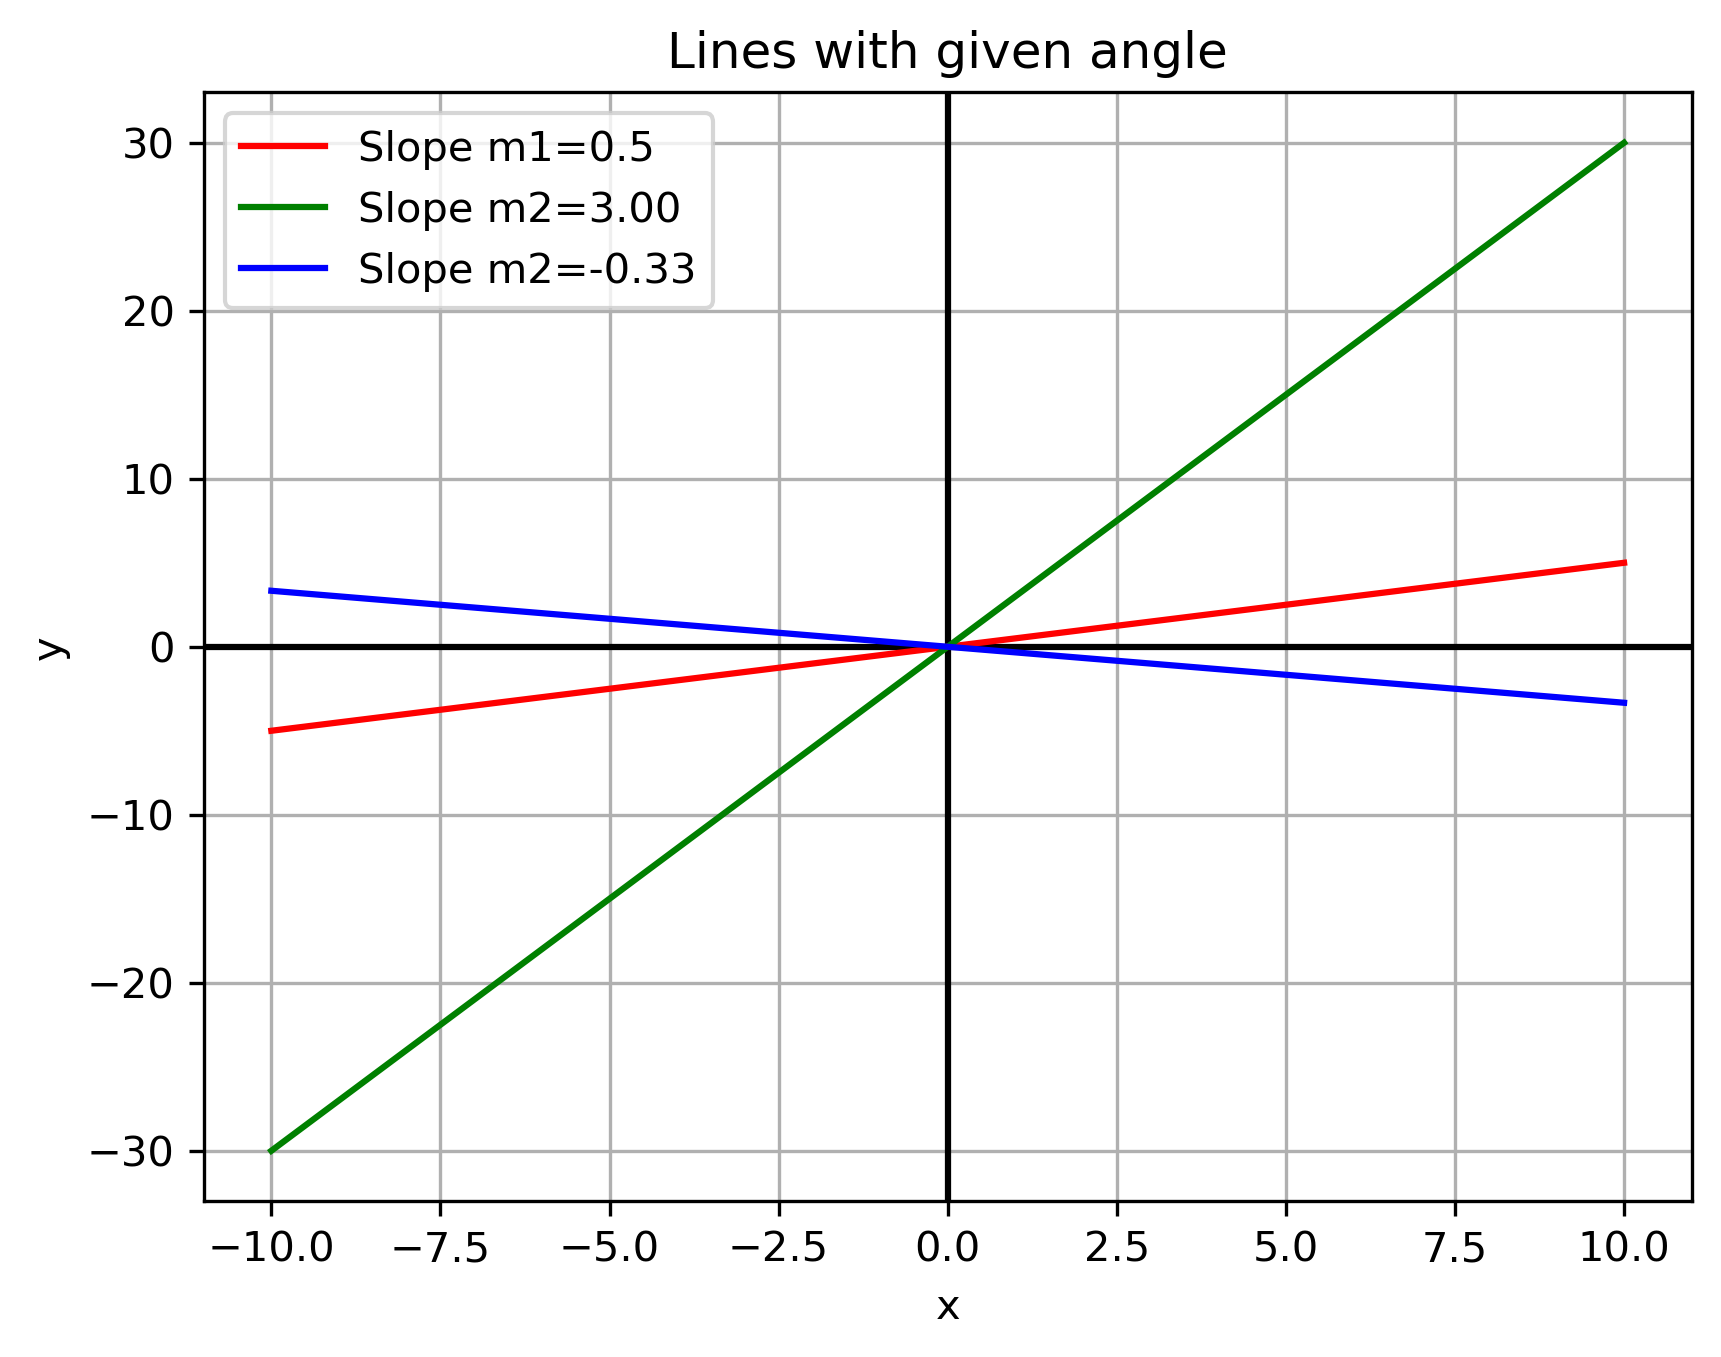
\includegraphics[width=\columnwidth, height=0.8\textheight, keepaspectratio]{figs/figure_1.png}     
\end{frame}

\begin{frame}[fragile]
    \frametitle{Python Code}
    \begin{lstlisting}
import numpy as np
import matplotlib.pyplot as plt

# === Vector analysis functions ===
def magnitude(v):
    return np.sqrt(v.T @ v)   # sqrt(v^T v)

def is_parallel(v, u, tol=1e-9):
    """Check if v is parallel to u. Return scalar t if v = t u, else None."""
    if np.allclose(u, 0):   # u is zero vector
        return None
    ratios = []
    for vi, ui in zip(v, u):
        if abs(ui) > tol:
            ratios.append(vi / ui)
        elif abs(vi) > tol:
            return None  # ui = 0 but vi != 0 --> not parallel
    


    \end{lstlisting}
\end{frame}

\begin{frame}[fragile]
    \frametitle{Python Code}
    \begin{lstlisting}
if len(ratios) == 0:
        return None
    t = ratios[0]
    if all(abs(r - t) < tol for r in ratios):
        return t
    return None

def dot_product(v, w):
    return v.T @ w   # v^T w

# === Example usage ===
v = np.array([2/3, -2/3, 1/3])
u = np.array([-1, 1, -0.5])
w = np.array([3, 2, -2])

# Analysis
mag_v = magnitude(v)
t = is_parallel(v, u)
dot_vw = dot_product(v, w)


    \end{lstlisting}
\end{frame}

\begin{frame}[fragile]
    \frametitle{Python Code}
    \begin{lstlisting}
    print("||v|| =", mag_v)
if t is None:
    print("v is NOT parallel to u")
else:
    print(f"v is parallel to u, scalar t = {t}")
print("v^T w =", dot_vw)

# === Plotting ===
fig = plt.figure(figsize=(6,6))
ax = fig.add_subplot(111, projection="3d")

origin = np.array([0,0,0])

# Draw vectors
ax.quiver(*origin, *v, color="r", linewidth=2, label="v")
ax.quiver(*origin, *u, color="g", linewidth=2, label="u")
ax.quiver(*origin, *w, color="b", linewidth=2, label="w")


    \end{lstlisting}
        
\end{frame}

\begin{frame}[fragile]
    \frametitle{Python Code}
    \begin{lstlisting}
    # Axes
ax.plot([0,1.5],[0,0],[0,0], color="k")
ax.plot([0,0],[0,1.5],[0,0], color="k")
ax.plot([0,0],[0,0],[0,1.5], color="k")
ax.text(1.6,0,0,"X",color="k")
ax.text(0,1.6,0,"Y",color="k")
ax.text(0,0,1.6,"Z",color="k")
ax.set_xlim([-1.5,1.5])
ax.set_ylim([-1.5,1.5])
ax.set_zlim([-1.5,1.5])
ax.set_xlabel("X-axis")
ax.set_ylabel("Y-axis")
ax.set_zlabel("Z-axis")
ax.legend()

     # Save before show
plt.savefig("/storage/emulated/0/matrix/Matgeo/2.10.17/figs/Figure_1.png", dpi=300, bbox_inches='tight')
plt.show()   
    \end{lstlisting}
\end{frame}
\end{document}
